\section{Piecewise (bi-)linear functions on multilevel grids}\label{sec:functions}
An image can be viewed as a function on a grid.  Images
with different resolutions can then be viewed as functions on grids of
different sizes.  The use of such multiple-grids is a main technique
used in the standard multigrid method for solving discretized partial
differential equations, 
and it can also be interpreted as a main ingredient used in
convolutional neural networks (CNN). 

Without loss of generality, for simplicity, we assume that the initial
grid, $\mathcal T$, is of size
$$
m=2^{s}+1~~~n=2^{t}+1 
$$
for some integers $t\ge 1$.
Starting from $\mathcal T_1=\mathcal T$,  we consider a sequence of
coarse grids (as depicted in Fig.~\ref{mgrid} with $J=4$):
\begin{equation}
\label{grids}
\mathcal T_1, \mathcal T_2, \ldots, \mathcal T_J
\end{equation}
such that ${\cal T}_\ell$ consist of $n_\ell\times n_\ell$ grid
points, with 
\begin{equation}
\label{mn-ell}
 m_\ell=2^{s-\ell+1}+1,~~ n_\ell=2^{t-\ell+1}+1.   
\end{equation}
\begin{figure}[!htbp]\label{mgrid}
	\begin{center}
		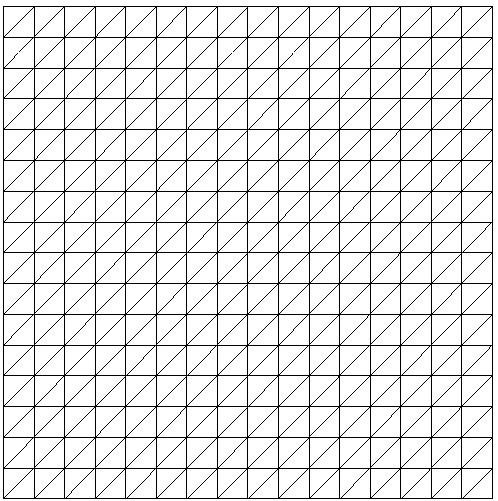
\includegraphics[width=0.15\textwidth]{grid2.png} \quad 
		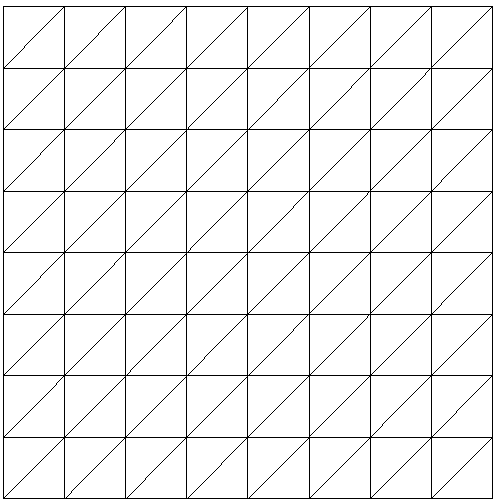
\includegraphics[width=0.15\textwidth]{grid1.png} \quad 
		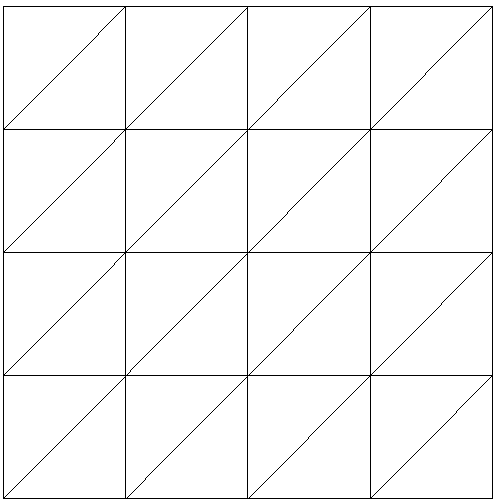
\includegraphics[width=0.15\textwidth]{grid0.png} \quad 
		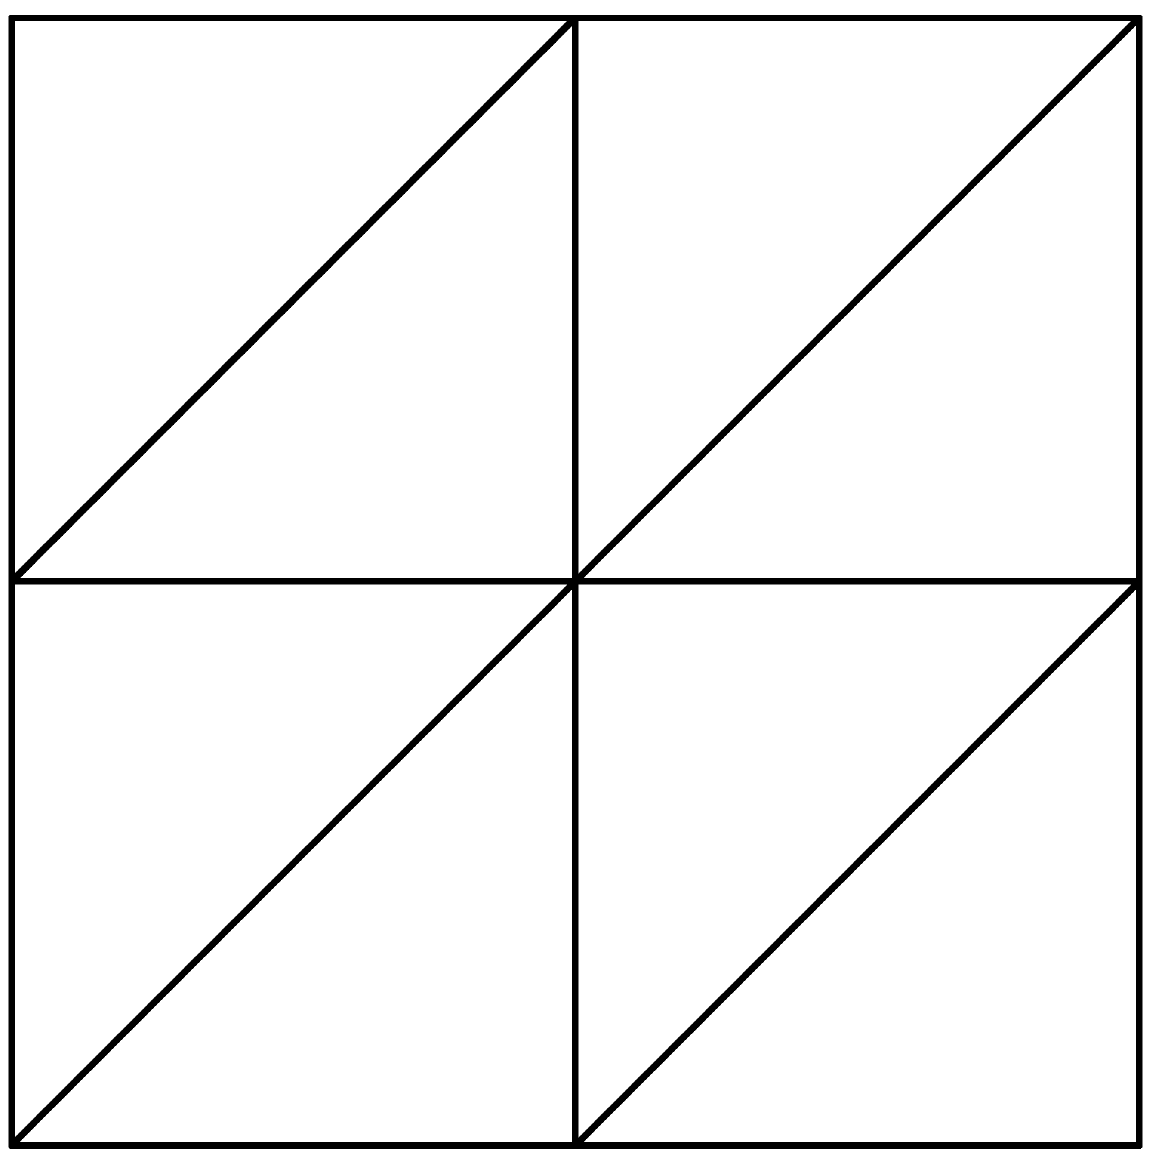
\includegraphics[width=0.15\textwidth]{grid.png} 
	\end{center}
	$$ 
	\mathcal T_1\hskip1in \mathcal T_2\hskip1in \mathcal T_3\hskip1in\mathcal T_4
	$$
	\caption{multilevel grids for piecewise linear functions}
\end{figure}

The grid points of these grids can be given by
$$
x_i^{\ell}=i h_{\ell}, y_j^{\ell}=j h_{\ell},  i=1, \ldots, m_\ell,
j=1, \ldots, n_\ell.
$$
Here $h_{\ell} = 2^{-s + \ell -1}a$ for some $a >0$. The above geometric coordinates $(x_i^\ell, y_i^\ell)$
are usually not used in image precess literatures, but they are relevant
in the context of multigrid method for numerical solution of PDEs.
We now consider piecewise linear functions on the sequence of grids
\eqref{grids} and we obtain a nested sequence of linear vector spaces
\begin{equation}
\label{Vk}
\mathcal V_1\supset\mathcal V_2\supset\ldots\supset \mathcal
V_J.
\end{equation}
Here each $\mathcal V_\ell$ consists of all piecewise bilinear (or linear)
functions with respect to the grid \eqref{grids} and \eqref{mn-ell}.
Each $\mathcal V_\ell $ has a set of basis functions:
$\phi_{ij}^\ell\in \mathcal V_\ell$ satisfying:
$$
\phi_{ij}^\ell(x_p,y_q)=\delta_{(i,j), (p,q)} = 
\begin{cases}
1 \quad &\text{if} \quad (p,q) = (i,j), \\
0 \quad &{\text{if}} \quad (p,q)\neq (i,j).
\end{cases}
$$
Thus, for each $v \in \mathcal V_{\ell}$, we have 
\begin{equation}\label{expand}
v(x,y)=\sum_{i=1}^{m_\ell}\sum_{j=1}^{n_\ell}v^\ell_{ij}\phi_{ij}^\ell(x,y).
\end{equation}

Let $\mathcal  V_1=\mathcal  V_h$, then the finite element method: Find $u_h\in \mathcal  V_h$ such that 
\begin{equation}\label{FEdis}
a(u_h, v_h)=(f, v_h)~~~\forall~~v_h\in \mathcal  V_h,
\end{equation}
where $a(u_h, v_h)=(\nabla u_h, \nabla v_h)$.
%\begin{lemma}
%FE $\rightarrow$ FD with $f_{i,j}=\int_{\Omega}f(x,y)\phi_{ij}(x,y)dxdy$.
%\end{lemma}

Finite element method: $A_h: \mathcal  V_h\rightarrow \mathcal  V_h, ~~(A_hu_h,v_h)_{L^2}=(\nabla u_h, \nabla v_h)$ (discrete Laplacian $A_h\approx -\Delta_h$. )
\begin{equation}\label{FE:eq}
A_hu_h=f_h,~~ 
\end{equation}
where~$f_h(x,y)=\sum_{i=1}^{m_1}\sum_{j=1}^{n_1}f_{i,j}\psi_{i,j}(x,y)$ and $\psi_{i,j}(x,y)\subset \mathcal V_h$ is also a basis, 
which is dual to the nodal basis $\phi_{ij}(x,y)$. namely $(\psi_{i,j}(x,y), \phi_{i,j}(x,y))_{L^2}=\delta_{(i,j), (p,q)}$.

The gradient descent for \eqref{FE:eq} is equivalent to the damped Jacobi method for \eqref{FE:eq} and can be written as follows 
$$
u^k=u^{k-1}+S_0(f-K_A\ast u^{k-1}),~~~1\le k\le m_1.
$$
Smoother  is equivalent to filter (filtering out high frequncies). Given any $u^0$, $u-u^k$ is much smoother than $u-u^0$. 

%Fine grid smoothing $\Longleftrightarrow$ feature extraction.

After smoothing, we do coarse grid correction: for example, for 
$\mathcal T_h,~\mathcal T_H,~H=2h, \mathcal V_2=\mathcal V_H\subset \mathcal V_h=\mathcal V_1$, we do
\begin{itemize}
\item $K_A\ast e=f- K_A\ast u^{m_1}=r^h$;
\item  $u=u^{m_1}+e$;
\item  $K_A\ast u=f$.
\end{itemize}
We need to solve the residual equation
$$
K_A\ast e=r^h.
$$
Multigrid idea: solve this residual  equation on coarse grid space $\mathcal V_H$ with $H=2h$ 

\subsection{Pooling or restriction}\label{sec:cnn-restriction}
Solving the residual equation 
$$
K_A\ast e=r^h
$$
in matrix form is equivalent to solve the problem 
\begin{equation}\label{FEres}
a(e_h, v_h)=(r_h,v_h)~~\forall~~v_h\in \mathcal V_h,
\end{equation}
where 
\begin{equation}\label{expresion:residual}
e_h=\sum_{i=1}^{m_1}\sum_{j=1}^{n_1}e^h_{i,j}\phi^h_{i,j}(x,y), r_h=\sum_{i=1}^{m_1}\sum_{j=1}^{n_1}r^h_{i,j}\psi^h_{i,j}(x,y).
\end{equation}
We solve the equation \eqref{FEres} on the coarse grid space $\mathcal V_H$, namely 
\begin{equation}\label{FEres:coarse}
a(e_{2h}, v_{2h})=(r_h,v_{2h})~~\forall~~v_{2h}\in \mathcal V_{2h},
\end{equation}
where $e_{2h}=\sum_{i=1}^{m_2}\sum_{j=1}^{n_2}e^{2h}_{i,j}\phi^{2h}_{i,j}(x,y)$, the matrix form for \eqref{FEres:coarse} is 
\begin{equation}\label{coarse:matrix}
K_A\ast e^{2h}=r^{2h},~~r_{i,j}^{2h}=(r_h,\phi^{2h}_{i,j})
\end{equation}
\begin{equation}\label{restriction}
r_{i,j}^{2h}=(r_h,\phi^{2h}_{i,j})
\end{equation}
Now we consider the expression of nodal basis functions $(\phi_{i,j}^{2h})(x,y)\subset \mathcal V_{2h}$ 
by the nodal basis functions $(\phi_{i,j}^{h})(x,y)\subset \mathcal V_{h}$. Here, we only show the details of the case of 
bilinear finite element space. The case of linear finite element space can be shown similarly. 
\begin{equation}\label{basis:plongation}
\begin{split}
\phi_{i,j}^{2h}(x,y)&=\phi_{2i,2j}^{h}(x,y)+\frac{1}{2}\left(\phi_{2i-1,2j}^{h}(x,y)+\phi_{2i,2j-1}^{h}(x,y)
+\phi_{2i+1,2j}^{h}(x,y)+\phi_{2i,2j+1}^{h}(x,y)\right)\\
&+\frac{1}{4}\left(\phi_{2i-1,2j-1}^{h}(x,y)+\phi_{2i+1,2j-1}^{h}(x,y)
+\phi_{2i+1,2j+1}^{h}(x,y)+\phi_{2i-1,2j+1}^{h}(x,y)\right)
\end{split}
\end{equation}


\subsection{Convolution with stride by introducing stride operator}
As discussed above, the restriction mapping is consistent with the 
co-called convolution with stride $s=2$, which is defined as:
\begin{equation}\label{stride_2}
[K \ast_2 f]_{i,j} = \sum_{p,q=-k}^k K_{p,q} f_{2i + p, 2j + q},  
\quad i = 1: \frac{m+1}{2} , j = 1: \frac{n+1}{2}.
\end{equation}


\begin{remark}
More generally in CNN, given an integer $s\ge1$, a convolution with stride $s$ for $f \in \mathbb{R}^{(m)\times
		(2^n+1)}$ can also be defined as:
	\begin{equation}\label{stride}
	[K \ast_s f]_{i,j} = \sum_{p,q=-k}^k K_{p,q} f_{si + p, sj + q},  
	\quad i = 1: \lceil  \frac{m}{s}\rceil , j = 1: \lceil  \frac{n}{s}\rceil.
	\end{equation}
	
	Here $ \lceil  \frac{m}{s}\rceil$ denotes the smallest integer that greater than $\frac{m}{s}$.
\end{remark}

As general in CNN and multigrid method, convolution with stride $s=2$ is the most important case.
To make this operator more clear, now we are going to introduce the stride operator $\mathcal S$ as:
\begin{equation}\label{eq:strideopdim}
\mathcal S: \mathbb{R}^{m \times n} \mapsto \mathbb{R}^{\frac{m+1}{2} \times \frac{n+1}{2}},
\end{equation}
with
\begin{equation}\label{eq:strideop}
[\mathcal S(f)]_{i,j} = f_{2i, 2j}, \quad i  = 1:\frac{m+1}{2}, j = 1:\frac{n+1}{2}.
\end{equation}

Then we have the rewrite form of convolution with stride $2$ as:
\begin{equation}\label{eq:convstride_2_1}
K \ast_2 f = \mathcal S( K\ast f).
\end{equation}


Then the deconvolution in defined by the transposed of convolution 
with stride with respect to the F-inner product defined as:
$$
(u, v)_F := \sum_{i,j} u_{i,j}v_{i,j}.
$$
Then we have the definition of deconvolution as
\begin{equation}\label{eq:def_deconv}
(K \ast_2 u, v)_F = (u, K \ast_2^\top v),
\end{equation}
with
\begin{equation}
u \in \mathbb{R}^{m \times n} \quad \text{and} \quad v \in \mathbb{R}^{\frac{m+1}{2} \times \frac{m+1}{2}}.
\end{equation}

For a more comprehensive notation, let us also define 
$K\ast$ as an operator from $\mathbb{R}^{m\times n} \quad \text{and}$
to $\mathbb{R}^{m\times n}$ as $\mathcal C_K$.
Then we have the ``transpose'' of convolution without stride as:
\begin{equation}\label{eq:def_tran_conv}
(K \ast u, v)_F = (\mathcal C_K (u), v) =  (u,  \mathcal C_K^\top v).
\end{equation}

\begin{lemma}\label{lemm:tilde-K}
For the transposed convolution without stride, we have the next result
\begin{equation}\label{eq:}
\mathcal C_K^\top = \mathcal C_{\tilde K},
\end{equation}
where $\tilde K$ is defined as
\begin{equation}\label{eq:def_tildeK}
\tilde K_{p,q} = K_{-p, -q}, \quad p,q = -k:k.
\end{equation}
Intuitively, if we take $K_{0,0}$ as the center for the convolutional kernel $K$, 
then $\tilde K$ is the central symmetry of $K$. 
In 2D case, it can also be understood as the rotation of $\pi$ with respect to
the center $K_{0,0}$.
\end{lemma}

Then recall the definition of deconvolution in \eqref{eq:def_deconv} we have
\begin{equation}\label{eq:op_deconv}
\begin{aligned}
(u,  K \ast_2^\top v) &= (K \ast_2 u, v)_F = (\mathcal S \mathcal C_K u, v) \\
&= (u,  \mathcal C^\top_K \mathcal S^\top v),
\end{aligned}
\end{equation}
with definition
\begin{equation}\label{eq:de_stride_dim}
\mathcal S^\top:   \mathbb{R}^{\frac{m+1}{2} \times\frac{n+1}{2}} \mapsto \mathbb{R}^{m\times n},
\end{equation}
and 
\begin{equation}\label{eq:de_stride}
[\mathcal S^\top (f)]_{i,j} = 
\begin{cases}
0 \quad &\text{if i or j is even}, \\
f_{i/2, j/2}, \quad &\text{else}.
\end{cases}
\end{equation}

Thus to say, we have the simple version of the deconvolution for $K \ast $ as
\begin{equation}\label{eq:simple_deconv}
K \ast_2^\top v = \mathcal C_K\top \circ \mathcal S^\top (v) = \mathcal C_{\tilde K} \circ \mathcal S^\top (v) = \tilde K \ast \mathcal S^\top (v),
\end{equation}
thus to say
\begin{equation}\label{eq:final}
K \ast_2^\top  = \tilde K \ast \mathcal S^\top.
\end{equation}

In short, we have the next decomposition
\begin{itemize}
	\item convolution with stride = stride $ \circ$ convolution,
	\item deconvolution with stride  = transposed convolution $\circ$ transposed stride = convolution with the central symmetry of original kernel $\circ$ transposed stride.
\end{itemize}

\begin{theorem}\label{thm:deconv_op}
Here let us show a simple example about some details for computing deconvolution. 
Let us consider 
\begin{equation}
K_{p,q} \quad p,q = -1, 0, 1.
\end{equation}
Then we have 
$$
K \ast_2^\top v = \tilde K \ast \mathcal S^\top (v).
$$
As in \eqref{eq:de_stride} and the Lemma \ref{lemm:tilde-K}, we have the 
final version is 
\begin{equation}
\label{eq:7}
[K \ast_2^\top v ]_{2i,2j}=  K_{0,0}v_{i,j},
\end{equation}
with 
\begin{equation}
\label{eq:9}
[K \ast_2^\top v ]_{2i-1, 2j} = K_{0,1}v_{i-1,j} + K_{0,-1}v_{i,j}, \quad 
[K \ast_2^\top v ]_{2i, 2j-1} = K_{1,0}v_{i,j} + K_{-1,0}v_{i,j-1},
\end{equation}
and
\begin{equation}
%\begin{tiny}
%{\scriptsize 
[K \ast_2^\top v ]_{2i-1, 2j-1}  =  
K_{1,1}v_{i,j} + K_{-1,1}v_{i-1,j} + K_{1,-1}v_{i,j-1} + K_{-1,-1}v_{i-1,j-1}.
%\end{tiny}
%}
\end{equation}


\end{theorem}


\subsection{Prolongation under the convolution notation}
Denote $\phi^h=\{\phi^h_{i,j}\}\in \mathbb R^{m_1\times n_1}$, 
by the definitions of convolution \eqref{con1} and stride \eqref{stride}, \eqref{basis:plongation} means that 
$$
 \phi^{2h}=K_R\ast_2 \phi^{h},
$$
where 
\begin{equation}\label{bi-restrict}
	K_R=
	\begin{pmatrix}
	\frac{1}{4} &\frac{1}{2}&\frac{1}{4}\\
	\frac{1}{2}& 1&\frac{1}{2}\\
	\frac{1}{4}&\frac{1}{2}&  \frac{1}{4} 
	\end{pmatrix}.
	\end{equation}
Now we derivatve of restriction and prolongation as follows. 

Let $r_{i,j}^{2h}=(r_h,\phi^{2h}_{i,j})_{L^2(\Omega)}$, then we have
\begin{equation}
\begin{split}
 r^{2h}&=\int_{\Omega} r_h \phi^{2h}=\sum\limits_{i=1}^{m_1}\sum\limits_{j=1}^{n_1}\int_{\Omega}r_{i,j}^{h}\psi_{i,j}(K_R\ast_2) \phi^h
=\sum\limits_{i=1}^{m_1}\sum\limits_{j=1}^{n_1}r_{i,j}^{h}(K_R\ast_2)\int_{\Omega}\psi_{i,j} \phi^h\\
&=\sum\limits_{i=1}^{m_1}\sum\limits_{j=1}^{n_1}(K_R\ast_2)r_{i,j}^{h}e_ie_j=K_R\ast_2 r^{h}.
\end{split}
\end{equation}
Hence the restriction 
$$
R^{2h}_h: \mathbb R^{m_{1}\times n_{1}}\mapsto  \mathbb R^{m_{2}\times n_{2}} 
$$
is obtain by $R^{2h}_h  r^{h}= K_R\ast_2  r^{h}$, namely
\begin{equation}\label{restriction:freedom}
\begin{split}
r_{i,j}^{2h}&=r^{h}_{2i,2j}+\frac{1}{2}(r^{h}_{2i-1,2j}+r^{h}_{2i,2j-1}+r^{h}_{2i+1,2j}+r^{h}_{2i,2j+1})\\
&+\frac{1}{4}\left(r^{h}_{2i-1,2j-1}+r^{h}_{2i+1,2j-1}+r^{h}_{2i+1,2j+1}+r^{h}_{2i-1,2j+1}\right).
\end{split}
\end{equation}
. 

Next 
let $u_{2h}=\sum\limits_{i=1}^{m_2}\sum\limits_{j=1}^{n_2}u_{i,j}^{2h}\phi^{2h}_{i,j}=( u^{2h}, \phi^{2h})_{l^2}$, then we have
\begin{equation}
%\begin{split}
u_{2h}=( u^{2h}, \phi^{2h})_{l^2}
=( u^{2h}, K_R\ast_2\phi^{h})_{l^2}=(K_R\ast_2^{\top} u^{2h}, \phi^{h})_{l^2}.
%\end{split}
\end{equation}
Thus the prolongation $P_{2h}^h u^{2h}=K_R\ast_2^{\top} u^{2h}$. Therefore by the definition of $K_R$ and equations 
\eqref{eq:7} and \eqref{eq:9} for the expression of $K_R\ast_2^{\top}$, we have 
 the prolongation 
$$
P_{2h}^h: \mathbb R^{m_{2}\times n_{2}}\mapsto  \mathbb R^{m_{1}\times n_{1} }
$$
is defined by 
$$
u^h_{2i,2j}=u^h_{i,j},
$$
$$
u^h_{2i-1,2j}=\frac{1}{2}(u^h_{i,j}+u^h_{i-1,j}),~~~ u^h_{2i,2j-1}=\frac{1}{2}(u^{2h}_{i,j}+u^{2h}_{i,j-1})
$$
and 
$$
u^h_{2i-1,2j-1}=\frac{1}{4}(u^{2h}_{i,j}+u^{2h}_{i-1,j}+u^{2h}_{i-1,j-1}+u^{2h}_{i,j-1}).
$$
In summery, for general $\mathcal V_1=\mathcal  V_\ell,  \mathcal V_2=\mathcal  V_{\ell+1}$, we have the restriction and prolongation
as follows: 
\begin{lemma}\label{ris:plon}
The restriction 
$$
R^{\ell+1}_\ell: \mathbb R^{m_\ell\times n_\ell}\mapsto  \mathbb R^{m_{\ell+1}\times n_{\ell+1}}~~\hbox{is}~~ R^{\ell+1}_\ell = K_R\ast_2  
$$ 
and the prolongation
$$
P_{\ell+1}^{\ell}: \mathbb R^{m_{\ell+1}\times n_{\ell+1}}\mapsto  \mathbb R^{m_{\ell}\times n_{\ell} } ~~\hbox{is}~~ P^{\ell}_{\ell+1} =K_R\ast_2^{\top} 
$$
where 
\begin{equation}\label{bi-restrict}
	K_R=
	\begin{pmatrix}
	\frac{1}{4} &\frac{1}{2}&\frac{1}{4}\\
	\frac{1}{2}& 1&\frac{1}{2}\\
	\frac{1}{4}&\frac{1}{2}&  \frac{1}{4} 
	\end{pmatrix}.
	\end{equation}
	for bilinear finite element space or 
\begin{equation}\label{li-restrict}
	K_R=
	\begin{pmatrix}
	0&\frac{1}{2}&\frac{1}{2}\\
	\frac{1}{2}& 1&\frac{1}{2}\\
	 \frac{1}{2} &\frac{1}{2}& 0
	\end{pmatrix}.
	\end{equation}	
for bilinear finite element space.	
\end{lemma}





	
	

